\documentclass[tikz,border=2mm]{standalone}
\usepackage{tikz}
\usetikzlibrary{arrows.meta,decorations.markings}

\begin{document}
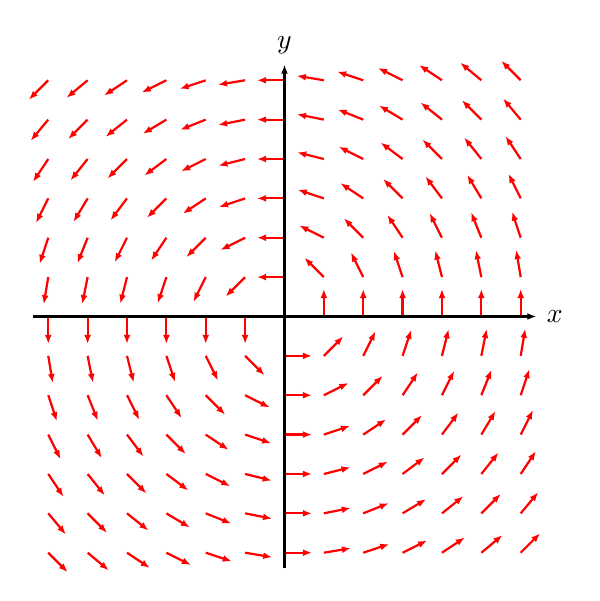
\begin{tikzpicture}[scale=1]
  % parameters
  \def\rmax{3}       % maximum radius
  \def\d{0.5}        % grid spacing
  \pgfmathsetmacro{\n}{int(\rmax/\d)}  % number of steps

  % draw vector field v = (-y, x) (unit-length scaled)
  \foreach \i in {-6,-5,...,6} {
    \foreach \j in {-6,-5,...,6} {
      \pgfmathsetmacro{\x}{\i*\d}
      \pgfmathsetmacro{\y}{\j*\d}
      \pgfmathsetmacro{\r}{sqrt(\x*\x+\y*\y)}
      \ifdim \r pt>0pt
        \pgfmathsetmacro{\vx}{- \y / \r}
        \pgfmathsetmacro{\vy}{  \x / \r}
        \pgfmathsetmacro{\len}{0.35}
        \draw[thick, -{Latex[scale=0.5]}, red] 
          (\x,\y) -- ++({\vx*\len},{\vy*\len});
      \fi
    }
  }

  % axes
  \draw[thick, -{Latex[scale=0.5]}] (-\rmax-0.2,0) -- (\rmax+0.2,0) node[right] {$x$};
  \draw[thick, -{Latex[scale=0.5]}] (0,-\rmax-0.2) -- (0,\rmax+0.2) node[above] {$y$};
\end{tikzpicture}
\end{document}
